\documentclass[a4paper,12pt,twoside]{article}

\usepackage[ngerman,english]{babel}

%%% FOR DISPLAYING CODE
\usepackage[procnames]{listings}
\usepackage{xcolor}

%%% MARGINS
\usepackage{geometry}
% INFO: https://www.overleaf.com/learn/latex/Page_size_and_margins
\geometry{
	a4paper,
%	total={170mm,257mm},
	left=25mm,
	top=25mm,
	textwidth=16cm,
	textheight=23cm,
%	right=25mm,
%	bottom=40mm,$
}

%%% SPACING
%\usepackage{setspace} 
%\onehalfspacing

\usepackage{siunitx} % for writing numbers with units % e.g. \SI{6.3e8}{km}, \ang{62.59}, \num{100}'s \si{km}, \SI{53}{\degree}
\usepackage{amsmath,amssymb}
\usepackage{graphicx}
\usepackage{datetime} 
\usepackage{color}
\usepackage{float} %without it, tables position more or less random, with this an writing \begin{table}[H] the table appears right where it is defined!
\usepackage{mathptmx}
\usepackage{enumitem}

\usepackage[T1]{fontenc}
\usepackage[utf8]{inputenc}

\usepackage{pgfplots} % for plotting functions
\pgfplotsset{compat=1.16}

%%% HEADER and FOOTER
%\usepackage[automark,headsepline]{scrpage2}
%\ihead[]{\headmark}
%\chead[]{}
%\ohead[]{\pagemark}
%\ifoot[]{}
%\cfoot[\pagemark]{}
%\ofoot[]{}
%\pagestyle{scrheadings}

\usepackage{lipsum}

%% LINE SPACING
\usepackage{setspace}
\setstretch{1.5}

%%% HYPERLINKS
\usepackage{hyperref} % muss sich vor cite stuff befinden

%% SET IMAGE PATH (where images are stored)
\graphicspath{{figures/}}

%%% CITE
\usepackage{apacite}
\bibliographystyle{apacite}

%%%%%%%%%%%%%%%%%%%%%%%%%%%%%%%%%%
% DEFINE COLORS
\definecolor{red}{rgb}{0.6,0,0} 
\definecolor{blue}{rgb}{0,0,0.6}
\definecolor{green}{rgb}{0,0.8,0}
\definecolor{cyan}{rgb}{0.0,0.6,0.6}

\definecolor{mypink}{rgb}{0.753,0.000,0.890}
\definecolor{myblue}{rgb}{0.078,0.000,1.000}
\definecolor{mybluedark}{rgb}{0.004,0.024,0.525} \definecolor{mygreen}{rgb}{0.000,0.514,0.000}
\definecolor{myreddark}{rgb}{0.698,0.000,0.008}
\definecolor{mycyan}{rgb}{0.000,0.506,0.612}
\definecolor{mybrown}{rgb}{0.494,0.365,0.090}

%%% DISPLAY CODE
\usepackage{listings}
\newcommand\pythonstyle{\lstset{
    language=Python,
	tabsize=4,
	basicstyle=\normalsize\sffamily,
	numberstyle=\color{gray},
	stringstyle=\color{myreddark},
    commentstyle=\color{mygreen},
    % KEYWORDS
    % main keywords
	keywordstyle=\normalsize\color{myblue},%\bfseries,
    % add keywords (main blue)
    emph={False,None,True,self,TODO},
    emphstyle={\color{myblue}},
    % pink emph
    emph={[2]assert,break,continue,del,elif ,else,except,finally,for,from,global,if,import,in,pass,raise,return,try,while,with,yield},
    emphstyle={[2]\color{mypink}},%\bfseries,
    %dark blue emph
    emph={[3]execfile,reduce,xrange},
    emphstyle={[3]\color{mybluedark}},
    % brown emph
    emph={[4]exec,print,isinstance,zip,enumerate,reversed,len,repr},
    emphstyle={[4]\color{mybrown}},
    % cyan emph
    emph={[5]object,type,list,set,dict,tuple,str,super},
    emphstyle={[5]\color{mycyan}},
    % errors (also cyan emph)
    emph={[6]Exception,NameError,IndexError,SyntaxError,TypeError,ValueError,OverflowError,ZeroDivisionError},
    emphstyle={[6]\color{mycyan}},
    % errors (also cyan emph)
    emph={[7]copy,deepcopy,append,real,imag},
    emphstyle={[7]\color{black}},
    % 
    showstringspaces=false,
	breaklines=true,
	numbers=left,
    frame=tb,
	xleftmargin=15pt
}}

\newcommand\javascriptstyle{\lstset{
	basicstyle=\small\sffamily,
    keywordstyle=\color{blue}\bfseries,
    commentstyle=\color{purple}\ttfamily,
    stringstyle=\color{red}\ttfamily,
	numberstyle=\color{gray},
    keywords={typeof, new, true, false, catch, function, return, null, catch, switch, var, if, in, while, do, else, case, break},
    ndkeywords={class, export, boolean, throw, implements, import, this},
    ndkeywordstyle=\color{darkgray}\bfseries,
    identifierstyle=\color{black},
    comment=[l]{//},
    morecomment=[s]{/*}{*/},
    morestring=[b]',
    morestring=[b]",
    showstringspaces=false,
	breaklines=true,
	numbers=left,
    frame=tb,
	xleftmargin=15pt,
    sensitive=false,
}}

\newcommand\csharpstyle{\lstset{
	language=csh,
	tabsize=4,
	basicstyle=\small\sffamily,
	numberstyle=\color{gray},
	stringstyle=\color{myreddark},
    commentstyle=\color{mygreen},
	morecomment=[l]{//}, %use comment-line-style!
	morecomment=[s]{/*}{*/}, %for multiline comments
    % KEYWORDS
	keywordstyle=\normalsize\color{myblue},%\bfseries,
	morekeywords={ abstract, event, new, struct,
		as, explicit, null, switch,
		base, extern, object, this,
		bool, false, operator, throw,
		break, finally, out, true,
		byte, fixed, override, try,
		case, float, params, typeof,
		catch, for, private, uint,
		char, foreach, protected, ulong,
		checked, goto, public, unchecked,
		class, if, readonly, unsafe,
		const, implicit, ref, ushort,
		continue, in, return, using,
		decimal, int, sbyte, virtual,
		default, interface, sealed, volatile,
		delegate, internal, short, void,
		do, is, sizeof, while,
		double, lock, stackalloc,
		else, long, static,
		enum, namespace, string},
	% 
    showstringspaces=false,
	breaklines=true,
	numbers=left,
    frame=tb,
	xleftmargin=15pt	
}}

% Python environment
\lstnewenvironment{python}[1][]
{
	\pythonstyle
	\lstset{#1}
}
{}
\lstnewenvironment{javascript}[1][]
{
	\javascriptstyle
	\lstset{#1}
}
{}
\lstnewenvironment{csharp}[1][]
{
	\csharpstyle
	\lstset{#1}
}
{}

% CODE FOR EXTERNAL FILES
\newcommand\pythonexternal[2][]{{
		\pythonstyle
		\lstinputlisting[#1]{#2}}}

% CODE FOR INLINE
\newcommand\pythoninline[1]{{\pythonstyle\lstinline!#1!}}
\newcommand\csharpinline[1]{{\csharpstyle\lstinline!#1!}}
\newcommand\javascriptinline[1]{{\javascriptstyle\lstinline!#1!}}

%% DEFINE CUSTOM COMMANDS AND SHORTCUTS

% some commands
\def\ba#1\ea{\begin{align}#1\end{align}}
\def\bas#1\eas{\begin{align*}#1\end{align*}}
\def\bmat#1\emat{\begin{pmatrix}#1\end{pmatrix}}
\newcommand{\ve}[1]{\vec{#1}}
\newcommand{\veTwo}[2]{\begin{pmatrix}#1\\#2\end{pmatrix}}
\newcommand{\veThree}[3]{\begin{pmatrix}#1\\#2\\#3\end{pmatrix}}
\newcommand{\veFour}[4]{\begin{pmatrix}#1\\#2\\#3\\#4\end{pmatrix}}
\newcommand{\ora}[1]{\overrightarrow{#1}}
\newcommand{\ola}[1]{\overleftarrow{#1}}
\newcommand{\s}[1]{\sqrt{#1}}

\def \bit{\begin{itemize}\setlength\itemsep{0em}} %\vspace{-5mm}
	\def \eit{\end{itemize}}

\def \ben{\begin{enumerate}\setlength\itemsep{0em}} %\vspace{-5mm}
	\def \een{\end{enumerate}}

\def \N{\mathbb{N}}
\def \Z{\mathbb{Z}}
\def \Q{\mathbb{Q}}
\def \R{\mathbb{R}}
\def \C{\mathbb{C}}

\def \ra{\rightarrow}
\def \longra{\longrightarrow}
\def \Ra{\Rightarrow}
\def \Longra{\Longrightarrow}
\def \la{\leftarrow}
\def \longla{\longleftarrow}
\def \La{\Leftarrow}
\def \Longla{\Longleftarrow}

\def \lra{\leftrightarrow}
\def \longlra{\longleftrightarrow}
\def \Lra{\Leftrightarrow}
\def \Longlra{\Longleftrightarrow}

\def \l{\left}
\def \r{\right}

\def \a{\alpha}
\def \b{\beta}
\def \g{\gamma}

\def \c{\cdot}

\def \el{\in}
\def \notel{\notin}

\newcommand{\f}{\frac}

\def \q{\quad}
\newcommand{\p}{\phantom}

\def\bs#1\es{\begin{split}#1\end{split}}


\def \L{\mathbb{L}}




\begin{document}

%%%%%%%%%%%%%%%%%%%%%%%%%%%%%%%%%%%%%%%%%%%%%%%%%%%%%%%
%%%%%%%%%%%%%%%%%%%%%%%%%%%%%%%%%%%%%%%%%%%%%%%%%%%%%%%
%%%%%%%%%%%%%%%%%%%%%%%%%%%%%%%%%%%%%%%%%%%%%%%%%%%%%%%

%%% AB HIER ARBEITEN, WEITER OBEN NICHTS VERAENDERN
%%% Ausnahme: Einbinden weitere Pakete

\selectlanguage{ngerman} %% HIER SPRACHE EINSTELLEN! english, ngerman

\begin{titlepage}
	\clearpage\thispagestyle{empty}	
	\setstretch{1}
	
	\begin{minipage}[t]{\textwidth}
		\begin{minipage}[t]{0.5\textwidth}
			Zeynep Zülal Keskin\\
			Mattfeldstrasse 6\\
			9532 Rickenbach b. Wil\\
			077 277 43 77\\
			zekeskin@ksr.ch
		\end{minipage}
		\begin{minipage}[t]{0.5\textwidth}
			\begin{flushright}
				Kantonsschule Romanshorn\\
				Klasse 4Ma\\
				Maturaarbeit
			\end{flushright}
		\end{minipage}
	\end{minipage}
	
	\vspace{4cm}
	{
		\centering
		\Huge\bfseries N-Körper Problem\par
		\vspace{1cm}
		\includegraphics[width=0.15\textwidth]{example-image-1x1}\par
	}
	
	\vspace{9cm}	
	\noindent
    Fach: Physik, Mathematik, Informatik \noindent\\
	Betreuungsperson: Dr. Andreas Schärer\\
	Abgabetermin: 6. Januar 2025
	
\end{titlepage}

%%%%%%%%%%%%%%%%%%%%%%%%%%%%%%%%%%%%%%%%%%%%%%%%%%%%%%%
%%%%%%%%%%%%%%%%%%%%%%%%%%%%%%%%%%%%%%%%%%%%%%%%%%%%%%%
%%%%%%%%%%%%%%%%%%%%%%%%%%%%%%%%%%%%%%%%%%%%%%%%%%%%%%%

% \null\thispagestyle{empty}\clearpage

%%% ABSTRACT

\pagenumbering{roman}

\section*{Abstract}

Das N-Körper-Problem ist ein fundamentales Problem der Himmelsmechanik, das die Bewegung von N Massenpunkten unter gegenseitiger gravitativer Anziehung beschreibt. Diese Arbeit untersucht zwei verschiedene Simulationsmethoden für das N-Körper-Problem: die direkte Methode und den Barnes-Hut-Algorithmus. Ziel ist es, die Genauigkeit und Effizienz dieser Methoden zu analysieren und zu vergleichen.
%%%%%%%%%%%%%%%%%%%%%%%%%%%%%%%%%%%%%%%%%%%%%%%%%%%%%%%
%%%%%%%%%%%%%%%%%%%%%%%%%%%%%%%%%%%%%%%%%%%%%%%%%%%%%%%
%%%%%%%%%%%%%%%%%%%%%%%%%%%%%%%%%%%%%%%%%%%%%%%%%%%%%%%

%%% TABLE OF CONTENTS

%\null\thispagestyle{empty}\clearpage
\newpage
%\setcounter{page}{1}
\tableofcontents

\parindent=0pt
\parskip=6pt

\newpage

\pagenumbering{arabic}

%%%%%%%%%%%%%%%%%%%%%%%%%%%%%%%%%%%%%%%%%%%%%%%%%%%%%%%
%%%%%%%%%%%%%%%%%%%%%%%%%%%%%%%%%%%%%%%%%%%%%%%%%%%%%%%
%%%%%%%%%%%%%%%%%%%%%%%%%%%%%%%%%%%%%%%%%%%%%%%%%%%%%%%

\section{Einleitung}
Diese Arbeit befasst sich mit einem der grundlegendsten und komplexesten Probleme der Himmelsmechanik und -dynamik: dem N-Körper-Problem in der Physik. Dieses Problem ist nicht nur von theoretischem Interesse, sondern findet auch praktische Anwendungen in der Astronomie, Raumfahrt und vielen anderen Bereichen der Physik. Die zentrale Forschungsfrage dieser Arbeit lautet: Welche mathematischen und physikalischen Methoden können verwendet werden, um die Bewegung von N-Körpern zu beschreiben und zu verstehen? 
Das Ziel dieser Arbeit ist es, die Bewegung von N-Körpern zu definieren und umfassend zu analysieren. Dabei soll der physikalische Hintergrund dieses Problems beleuchtet und seine historische Entwicklung nachgezeichnet werden. Ein besonderer Schwerpunkt liegt auf der Darstellung und Untersuchung der verschiedenen mathematischen und physikalischen Methoden, die im Laufe der Zeit entwickelt wurden, um die Dynamik von N-Körpern zu erklären.
Darüber hinaus werden zwei detaillierte Simulationen entwickelt, um die theoretischen Konzepte praktisch zu veranschaulichen. Diese Simulationen dienen nicht nur der Erklärung des Problems, sondern auch dem Vergleich verschiedener Lösungsansätze. Durch diese Herangehensweise soll ein tieferes Verständnis für die Komplexität des N-Körper-Problems und die Herausforderungen bei seiner Lösung vermittelt werden.
Ein weiterer Aspekt dieser Arbeit ist die Untersuchung der praktischen Relevanz des N-Körper-Problems. Dabei wird aufgezeigt, wie die theoretischen Erkenntnisse in der Astronomie zur Berechnung von Planetenbahnen, in der Raumfahrt zur Planung von Satellitenmissionen und in anderen Bereichen der Physik zur Modellierung komplexer Systeme angewendet werden können.
Zusammenfassend strebt diese Arbeit an, einen umfassenden Überblick über das N-Körper-Problem zu geben, seine Bedeutung in der modernen Physik aufzuzeigen und durch die Entwicklung und den Vergleich von Simulationen einen Beitrag zur Lösung dieses faszinierenden und herausfordernden Problems zu leisten.

\newpage
\section{Theoretische Grundlagen}

\subsection{Problembeschreibung und historische Entwicklung}
Das N-Körper-Problem beschäftigt sich mit der dynamischen Analyse von N Massepunkten, die durch ihre gegenseitige gravitative Anziehung beeinflusst werden. Während das Zwei-Körper-Problem durch Newtons Gesetz der universellen Gravitation und die Keplerschen Gesetze exakt gelöst werden kann, wird das N-Körper-Problem für N Körper wesentlich komplexer und zeigt in der Regel chaotisches Verhalten. Die historische Entwicklung dieses Problems begann im 17. Jahrhundert mit den grundlegenden Arbeiten von Johannes Kepler und Isaac Newton, die die Basis für die Himmelsmechanik schufen. Im 18. und 19. Jahrhundert erweiterten Joseph-Louis Lagrange und Pierre-Simon Laplace das Verständnis durch die Einführung der Lagrangeschen Gleichungen und durch die Analyse spezieller Lösungen wie der Lagrange-Punkte, die besondere Gleichgewichtslagen in einem gravitativen System beschreiben. Henri Poincaré entdeckte Ende des 19. Jahrhunderts die chaotische Natur des Systems, was den Beginn der modernen Chaosforschung einleitete. Im 20. und 21. Jahrhundert ermöglichten Fortschritte in der Computertechnologie und numerischen Methoden präzise Simulationen und Analysen komplexer N-Körper-Systeme, die wichtige Einblicke in die Dynamik von Galaxien und die Planung von Raumfahrtmissionen bieten.

\subsection{Gravitationskraft}
Die Gravitationskraft $\vec{F}_{12}$ zwischen zwei punktförmigen Massen $m_1$ und $m_2$ liegt auf der Verbindungslinie der beiden Massen. Der Betrag $F$ der Gravitationskraft ist proportional zu den Massen $m_1$ und $m_2$ sowie umgekehrt proportional zum Quadrat des Abstands $r$ (die relative Position ist die Position eines Körpers relativ zu einem anderen: \(\mathbf{r} = \mathbf{r}_2 - \mathbf{r}_1\)) der Massen. Er berechnet sich durch:
\[
F = G \frac{m_1 m_2}{r^2}
\]
mit der Gravitationskonstante $G = 6{,}674 \times 10^{-11} \, \frac{\text{m}^3}{\text{kg s}^2}$.

\subsection{Zwei-Körper-Problem}

Das Zwei-Körper-Problem beschreibt in der klassischen Mechanik die Bewegung zweier Körper, die sich unter dem Einfluss einer zentralen Kraft (in der Regel die Gravitation) gegenseitig anziehen. Es ist ein fundamentales Problem der Himmelsmechanik und bildet die Grundlage für das Verständnis von Bahnbewegungen, wie sie z.B. bei Planeten, Satelliten oder Doppelsternsystemen auftreten.
Gegeben sind zwei Massen \( m_1 \) und \( m_2 \), die sich unter dem Einfluss ihrer gegenseitigen Gravitationskraft bewegen.
Ziel ist es, die Bewegungsgleichungen für beide Körper zu lösen und ihre Bahnen zu bestimmen.
\subsubsection{Schwerpunktsystem und Reduktion auf das Ein-Körper-Problem}
Um die Lösung des Problems zu vereinfachen, führt man ein Koordinatensystem ein, das den Schwerpunkt des Systems beschreibt. Der Schwerpunkt befindet sich an der Position:
\[
R_{\text{Schwerpunkt}} = \frac{m_1 r_1 + m_2 r_2}{m_1 + m_2}
\]
Durch die Transformation in das Schwerpunktsystem kann die Bewegung der beiden Körper auf die Bewegung eines Körpers mit der sogenannten reduzierten Masse \( \mu \) relativ zu einem der beiden Körper reduziert werden. Die reduzierte Masse wird durch:
\[
\mu = \frac{m_1 m_2}{m_1 + m_2}
\]
definiert. Die Bewegung dieses fiktiven Körpers wird durch eine Differenzialgleichung beschrieben, die sich aus dem zweiten Newtonschen Gesetz ableiten lässt:
\[
\mu \frac{d^2}{dt^2} = - G \frac{m_1 m_2}{r^2} 
\]
Dies ist die Grundgleichung des Zwei-Körper-Problems, die die Bewegung eines Körpers unter dem Einfluss der Gravitationskraft eines anderen Körpers beschreibt.
Nachdem die Beschleunigung bestimmt wurde, kann die Geschwindigkeit des Körpers durch die Formel \( \mathbf{v}(t) = \mathbf{v}_0 + \mathbf{a} t \) berechnet werden. Um die neue Position des Körpers zu berechnen, verwendet man die folgende Formel: \( \mathbf{r}(t) = \mathbf{r}_0 + \mathbf{v}_0 t + \frac{1}{2} \mathbf{a} t^2 \).

\subsubsection{Lösung der Bahnkurve}
Im Zweikörperproblem beschreibt der Abstand \( r \) die Distanz zwischen den beiden Massen \( m_1 \) und \( m_2 \) oder die relative Position eines Körpers zum Schwerpunkt des Systems. Der Winkel \( \theta \) gibt die Lage des Körpers auf seiner Umlaufbahn in Bezug auf eine feste Referenzachse an. In Polarkoordinaten wird die Bahn des Körpers durch die Gleichung:
\[
r(\theta) = \frac{p}{1 + e \cos(\theta)}
\]
beschrieben, wobei \( p \) der Bahnhalbmesser und \( e \) die Exzentrizität (ist ein Maß für die Abweichung von einer perfekten Kreisbahn: Sie liegt zwischen 0 (Kreis) und größer als 1 (Hyperbel). Diese Information ist entscheidend, um die Form und die Eigenschaften der Bahn zu verstehen) ist. Diese Parameter charakterisieren, ob die Bahn elliptisch, parabolisch oder hyperbolisch ist, wobei der Winkel \( \theta \) die Bewegung entlang der Bahn angibt.

\begin{figure}[H]
	\centering
	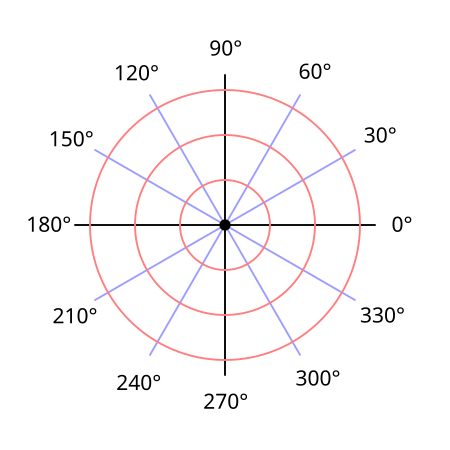
\includegraphics[width=0.4\textwidth]{Polarkoordinaten.svg.png}
	\caption[Eintrag in Abbildungsverzeichnis von Polarkoordinatsystem]{Polar koordinaten sind ein System zur Beschreibung der Position eines Punktes durch seinen Abstand vom Ursprung und den Winkel, den die Verbindungsgerade zum Ursprung mit einer festen Referenzachse bildet.}
	\label{polarkoordinatsystem.}
\end{figure}

\subsection{Drei-Körper-Problem}Im Gegensatz zum Zwei-Körper-Problem, das durch die Kepler-Gesetze vollständig analytisch lösbar ist, gibt es für das Drei-Körper-Problem keine allgemeine analytische Lösung. Das Problem beschreibt die Bewegung dreier Objekte (z.\,B.\ Sterne, Planeten oder Monde), die sich gegenseitig aufgrund der Gravitation anziehen. Jedes Objekt wird durch die resultierende Gravitationskraft der beiden anderen beeinflusst, was zu einer sehr komplizierten Dynamik führt.
Für das Zwei-Körper-Problem kann die Bewegung der beiden Objekte auf elliptische, parabolische oder hyperbolische Bahnen reduziert werden, je nach den Anfangsbedingungen. Das Drei-Körper-Problem hingegen führt oft zu unvorhersehbaren, chaotischen Bewegungen, außer in speziellen Fällen mit symmetrischen oder stark eingeschränkten Anfangsbedingungen.

\subsection{N-Körper Problem}

\section{Material und Methoden}
\subsection{Vorgehensweise und Implementierung}

\section{Resultat}
\subsection{Vergleich der Simulationsergebnisse}

\section{Diskussion}
\subsection{Vorteile der verwendeten Algorithmen}
\subsection{Herausforderungen und Limitierungen}
\subsection{Vergleich mit bestehenden Methoden}

\section{Schlussfolgerung}
\section{Literaturverzeichnis}
\section{Abbildungsverzeichnis}

\end{document}

